\documentclass[11pt]{amsart}
\usepackage{geometry}           % See geometry.pdf to learn the layout options. There are lots.
\geometry{letterpaper}          % ... or a4paper or a5paper or ... 
%\geometry{landscape}           % Activate for for rotated page geometry
%\usepackage[parfill]{parskip} 	% Activate to begin paragraphs with an 
								% empty line rather than an indent
\usepackage{graphicx}
\usepackage{amssymb}
\usepackage{epstopdf}
\usepackage{tikz-qtree}
\usepackage{enumitem}
\usepackage{natbib}

%---------------------- For System Architecture -------------------------------------------%
\usetikzlibrary{positioning,calc,fit}

\definecolor{mybluei}{RGB}{124,156,205}
\definecolor{myblueii}{RGB}{73,121,193}
\definecolor{mygreen}{RGB}{202,217,126}
\definecolor{mypink}{RGB}{233,198,235}

% this length is used to control the width of the light blue frame
% for the upper part of the diagram
\newlength\myframesep
\setlength\myframesep{8pt}

\pgfdeclarelayer{background}
\pgfsetlayers{background,main}

\pgfkeys{
  /tikz/node distance/.append code={
    \pgfkeyssetvalue{/tikz/node distance value}{#1}
  }
}

\newcommand\widernode[5][blueb]{
  \node[
    #1,
    inner sep=0pt,
    shift=($(#2.south)-(#2.north)$),
    yshift=-\pgfkeysvalueof{/tikz/node distance value},
    fit={(#2) (#3)},
    label=center:{\sffamily\bfseries\color{white}#4}] (#5) {};
}
%---------------------- End of System Architecture ----------------------------------------%

\DeclareGraphicsRule{.tif}{png}{.png}{`convert #1 `dirname #1`/`basename #1 .tif`.png}

\title{Proposition of Volunteer Cloud Computing}
\author{Dany Wilson}
%\date{}                                         % Activate to display a given date or no date

\begin{document}
\maketitle
	\section{Introduction}
	In this current era we can see a shift in how software and hardware are conceived, the end-
	goals are not the same as they used to be 2 decades ago. This can be attributed to the 
	following, the fact that the Internet speed got a lot faster, by a factor of 1000 (based on
	a 56kbps connection in 1995, compared to a 50mbps connection today), but also because the 
	hardware performance augmented at a similar pace. Initially in the pre-Internet era, 
	software was written to be executed locally without any network interactions. Then in the 
	genesis of the Internet, the objectives of software slowly shifted to access external 
	resources, thus the apparition of the e-mail and the web-browser. Slowly as the connection
	bandwidths increased, there was an increased number of possible usage such as online games, 
	content streaming, social-media, etc. Nowadays we can access fully virtualized computing
	environments within our web-browsers, and this takes us the very genesis of the Cloud 
	Computing era. 

	\subsection{The Genesis of Cloud Computing}
	The embodiment of Cloud Computing, namely the Internet of Things, can actually be traced 
	back to the vision of J.C.R. Licklider of the \emph{"Intergalactic Computer Network"} 
	\cite{licklider}:
	\begin{quote}
		At this extreme, the problem is essentially the one discussed by science fiction 
		writers: \emph{"how do you get communications started among totally uncorrelated 
		sapient beings?"}
	\end{quote}
	This quote shows us the state of electronic tele-communication in the sixties, which is 
	described as being fabric of fiction. There was military but also academic interest of 
	providing an infrastructure that supports long-distance information processing. One of the most 
	interesting idea of this memorandum is best conveyed in this following quote:
	\begin{quote}
		When the computer operated the programs for me, I suppose
		that the activity took place in the computer at SDC, which
		is where we have been assuming I was. However, I would just
		as soon leave that on the level of inference. With a
		sophisticated network-control system, I would not decide
		whether to send the data and have them worked on by
		programs somewhere else, or bring in programs and have them
		work on my data. I have no great objection to making that
		decision, for a while at any rate, but, in principle, it
		seems better for the computer, or the network, somehow, to
		do that.
	\end{quote}
	This very quote reflects the concept of offloading, not only of information or data, but 
	of computation as a service. In other words that in some case it would be better, given the 
	proper networking infrastructure, to offload the computation and send the data to be 
	processed remotely.
	
	Around the same time the concept of virtualization was being explored in the context of 
	mainframe computers, in order to logically divide the resources between applications 
	allowing them to run simultaneously. Throughout the years, the concept of virtualization 
	broaden and now it is possible to run a complete Operating System on the application level.
	There is a direct correlation with the coming of the virtualization of hardware and the 
	birth of the Cloud. 
	
	Cloud Computing is heavily influenced by the maturity of the Service-Oriented Architecture, 
	and as we said earlier the evolution of the "Internet" with respect to the Web 2.0. That 
	evolution of the Web from 1.0 to 2.0 is marked by the following characteristics, as cited in 
	\cite{web20}: \emph{[...] services, not packaged software, with cost-effective scalability; 
	[...] data-centric w.r.t. Big Data; [...] users as co-developers; [...] harnessing collective 
	intelligence; [...] leveraging long-tail effect through customer self-service.} We can observe 
	a trend, the concept (web) services (rather then serving only static content) but also how 
	the user becomes the central point of the network as a platform. This entails that components 
	of the Web are becoming interactive services that can be contracted to responds to the users 
	needs, via real-time aggregation of information using Big Data.

	Thus the Cloud is the natural evolution of utilizing the network as a platform, through a 
	Service-Oriented Architecture with respect to the natural evolution and maturity of the 
	Web entailing the definition and wide-spread usage of mature Web-Services homogeneous 
	interface (API). \emph{Ipso Facto}, the adoption of pay-per-use business model for the 
	offerings of Cloud Infrastructure.
	
	% Need to talk about its similarities between the SOA, distributed, grid computing...
	%
	\subsection{The Cloud}
	There have been numerous attempts to try to give a concise or approximate picture of the 
	Cloud Computing paradigm, with respect to its implementation and its different business 
	models. One can review the following, \cite{soa_cloud}, \cite{vaquero}, \cite{ontology},\cite{panzieri}; 
	to name a few. We feel that \cite{nist}, \cite{soa_cloud} and \cite{ontology}, provides a 
	clear enough picture to represent the current Cloud ecosystem and we will use them to do so.
		
	Cloud Computing infrastructure offers many advantages compared to the traditional on-premise 
	infrastructure and it is why numerous companies consider outsourcing their IT infrastructure to 
	an off-premise solution. Among the most important characteristics that this type of 
	infrastructure offers, the NIST enumerates the following five \cite{nist}:
	\begin{enumerate}
		\item{\textbf{On-demand Self-service}} \emph{Consumers are not required to interact with 
		any representative of the provider to provision computing capabilities, rather it is 
		automated through the provider's infrastructure.}\\
		\item{\textbf{Broad Network Access}} \emph{Services are available over standard network 
		infrastructure and through standard	mechanisms, enabling different client platforms like 
		cell-phones, laptop, tablets, etc.}\\
		\item{\textbf{Resource Pooling}} \emph{Providers offers a pool of Resources to different 
		clients via a multi-tenant model, consisting of physical and virtual resources that can be 
		assigned and re-assigned dynamically to cater to the clients demands. Clients are only 
		aware, or able to choose the location of these resources with respect to pre-defined 
		geographical regions. }\\
		\item{\textbf{Rapid Elasticity}} \emph{Resources and services can be provisioned to scale 
		to meet the fluctuations of the client's needs at any time, at any magnitude. The provider
		offers a seemingly unlimited number of services and resources to the client.}\\
		\item{\textbf{Measured Service}} \emph{Resource usage can be monitored, controlled 
		(optimized) and reported in a manner that proves transparent to both provider and consumer.}
	\end{enumerate}
	
	In this modern day and age, among the major service providers of \emph{The Cloud} we can 
	find the likes of Google, Microsoft and Amazon, to name a few. They provide their services 
	as a 5 different service models:\\
	
	\begin{center}
		% Cloud Services graphic (may need to represent it better...)
		\begin{figure}[h]
			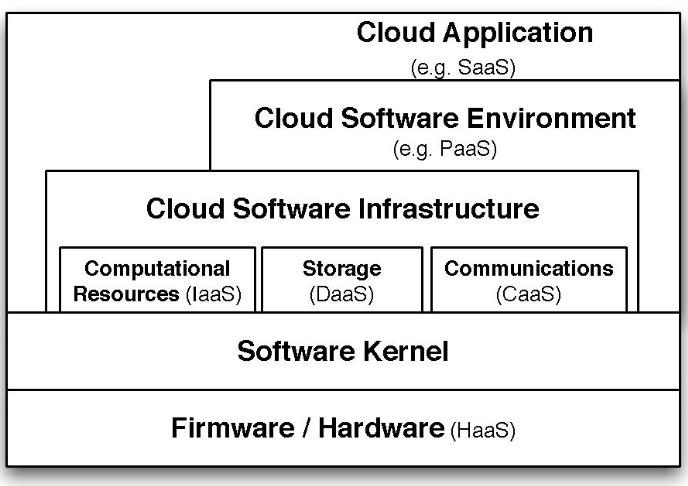
\includegraphics[width=125mm]{c_ontology.png}
			\caption{Ontological Representation of Cloud\label{c_ontology}}
		\end{figure}
	\end{center}
	
	Based on \cite{ontology}, we can appreciate the categorization that emerged from their study of 
	the major Cloud Service providers. We will briefly explain 3 of these categories in order to 
	have a clearer picture of where this proposition resides in the grand scheme of the Cloud. In 
	order to do so we will explore the question with respect of the Separation of Responsibilities, 
	via a very concise graphical depiction \cite{Blewis}:
	
	\begin{center}
		\begin{figure}[h]
			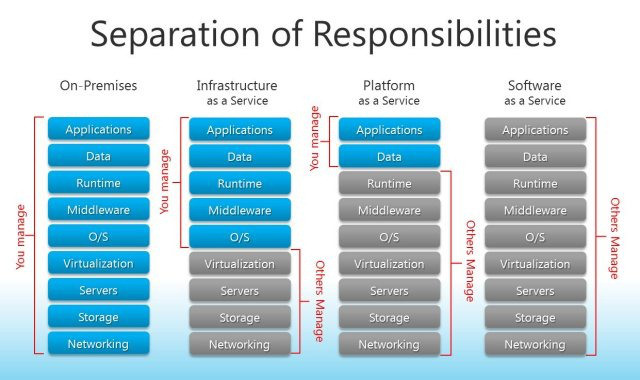
\includegraphics[width=125mm]{cloud_sep_of_resp.jpg}
			\caption{Cloud Services w.r.t. Responsibilities\label{cloud_sep_of_resp}}
		\end{figure}
	\end{center}
	
	\subsubsection{Infrastructure-as-a-Service (IaaS)}
	This service model provides, to its consumers, a virtualized environment that represents the 
	full stack, from the hardware-level to the software-level, while taking care of the hardware 
	management aspect. With this model, consumers can deploy any Operating System they wish, and as a
	matter of fact create the software environment that they deem most appropriate for their use. 
	Since the hardware management responsibility is left out to the service provider, the client can 
	easily augment or reduce the computing power at will to cope with the fluctuation of their 
	demands. Amazon's Elastic Cloud Compute (EC2), or Windows Azure are part of the available IaaS 
	solutions currently available.
	
	\subsubsection{Platform-as-a-Service (PaaS)}
	This service model, if we refer to Figure \ref{cloud_sep_of_resp}, to its clients the ability of 
	having to manage only the Application and Data aspect of the full-stack, everything else is \
	managed and taken care of by its provider. Using such a service the client can focus on simply 
	developing their application using the libraries, services and tools supported by the provider, 
	and then deploy it onto the Cloud. Google's App Engine is perhaps one of the most popular example 
	of this model.
	
	\subsubsection{Software-as-a-Service (SaaS)}
	This service model, the consumer is provided with the capability to use applications (or 
	software) running on the provider's cloud infrastructure, with little to no management 
	capability, as depicted in Figure \ref{cloud_sep_of_resp}. From a user's perspective application 
	are served as an atomic service, in the likes of Oracle ON DEMAND which offers on demand a 
	customer relationship management application.
	
	Finally we need to discuss the different \emph{Deployment Models} that are offered in the Cloud 
	eco-system. Relying again on the NIST \cite{nist} document, let's briefly present the 4 models:
	
	\begin{enumerate}
		\item{\textbf{Private Cloud}} \emph{This cloud infrastructure is meant to be used by a single 
		organization, which can act also as a single provider or a providing partner with a 3rd party 
		or solely as a consumer. Exclusivity is the key here.}\\
		\item{\textbf{Community Cloud}} \emph{Very similar to the private cloud model, but in this 
		case exclusivity of usage is shared among a community sharing common interests.}\\
		\item{\textbf{Public Cloud}} \emph{This deployment model is aimed for open use by the general 
		public, and the embodiment of this model's infrastructure is known as a Cloud Provider, such 
		as Amazon, Google, Windows, etc.}\\
		\item{\textbf{Hybrid Cloud}} \emph{This is the result of the combination of two or more 
		distinct cloud infrastructure (which remain distinct to one another), but are combined using 
		standardized or proprietary technologies to enable data and application portability.}
	\end{enumerate}
	
	In the following subsection we will present a fifth deployment model, namely Volunteer Cloud 
	Computing. But in order to provide the proper context for its emergence, lets take a brief look
	at Grid Computing and Volunteer Computing.
	
	\subsection{Grid Computing}
	A very extensive literature exist on this fairly recent paradigm (cite proper sources), and we 
	can define it as being a form of Distributed Computing, where each node is ask to perform a 
	different task, and the aggregation of those nodes workload constitutes the workload that needs 
	to be perform in order to achieve the goal of (computationally) realizing its mandate. A
	
	\subsection{Volunteer Computing}
	The @Home paradigm or philosophy beautifully proves how this is realized, and let's look at a 
	simple example the SETI@Home project.
	
	%mention panzieri for its representation of different cloud topologies.
	
	\subsection{Volunteer Cloud Computing}
	The concept of Volunteer Cloud Computing is a fairly new one, since as we can see there is no 
	mention of it whatsoever in \cite{nist}\cite{taxonomy}. It revolves around user-provided 
	resources as the building components of the cloud infrastructure, and typically takes place in 
	a decentralized manner for which no single provider is designated, rather the collection of the
	participants form at the same time the provider and the consumers. One of the driving factors of 
	this topological ideology is to harvest and make efficient use of distributed idling 
	resources to provide a cloud infrastructure, with no real added cost. 
	
	In the following section we will review the literature to find out more about the position of 
	Volunteer Cloud Computing with respect to the current deployment models in place, and if any 
	implementation exists.
	
	\section{Related Work}
	
	\subsection{Cloud@Home}
	The first real apparition of the term Volunteer Cloud Computing can be attributed to 
	\cite{cathome}, in 2009 when they proposed the Cloud@Home paradigm. It can be described as a 
	continuation of the @Home distributed computing effort and the merging of volunteer computing and 
	Cloud computing. They propose an infrastructure in which it is possible for heterogeneous 
	computing resources to be connected and to co-operatively provide a Cloud infrastructure, at a 
	cost or for free. Thus this is a leap into monetizing the idle time of the consumer-grade 
	computing resources, to provide a seamless Cloud experience to consumers. Although they provide a 
	very detail analysis of the majority of the factors present in a Cloud architecture, little to no 
	information was released after the publication of a series of more specific papers on the 
	subject,.
	%\cite{cathome2}.
	Last paper that was published, \cite{cathome11}, was indicating that they were actively working on 
	an implementation of their proposed framework, but that was back in 2012. Thus, we will elaborate 
	on what are the characteristics of this project, and try to understand why it seemed to have stop 
	or at least why the driving factors seems less violent as they once were.
	
	\subsubsection{Preliminaries}
	The complete bibliography of the project span over 11 papers, which a couple of them are re-publications 
	in different proceedings, journal, and/or conferences. The first paper \citet{cathome}, presents 
	an overview of the scope and motivation, which we already discussed, but also presents a tentative 
	architecture of what a it could become. What is very interesting here is the presentation of the 
	\emph{Issues, Challenges and Open Problems}, for which they define 6 aspects that will act a 
	mind-map of the problems to tackle along the way, as well as a reminders of the realizability of 
	some more open problems. Let's list them, as presented: 
	\begin{enumerate}
		\item{\textbf{Resources and Service Management:}}\emph{ Need for a mechanism that provides it.}
		\item{\textbf{Frontend:}}\emph{ Provide users with high-level service-oriented POV of the Cloud 
		Infrastructure.}
		\item{\textbf{Security:}}\emph{ Cite different security concerns, not important for now.}
		\item{\textbf{Reliability:}}\emph{ Need for redundancy, and recovery mechanisms.}
		\item{\textbf{Interoperability:}}\emph{ Need to operate with other Cloud Infrastructures.}
		\item{\textbf{Business Models:}}\emph{ Need for QoS/SLA management for commercial Clouds, and 
		also with the open volunteer Cloud framework.}
	\end{enumerate}
	
	\subsubsection{Architecture}
	Next they present an architecture that responds to these challenges (or requirements) partially 
	or fully, but in a abstract fashion. A picture is worth a 1000 words, thus let's not babble on this 
	much longer and present it: 
	
	% need to find the picture of the architecture and replace this dummy jpg!!!!
	\begin{center}
		\begin{figure}[h]
			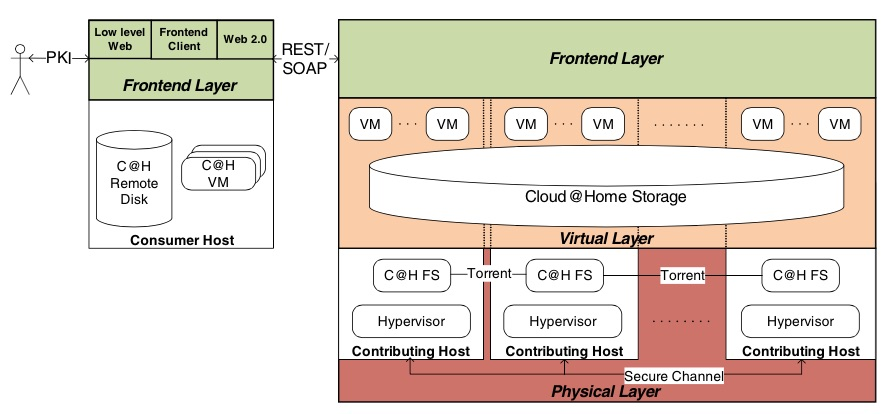
\includegraphics[width=125mm]{cathome_arch.jpg}
			\caption{Cloud@Home Architecture\label{cathome_arch}}
		\end{figure}
	\end{center}
	
	We can observe the three-tier approach to organize the architecture: \emph{Frontend Layer}, \emph{Virtual Layer} 
	and the \emph{Physical Layer}.
	\\
	The \textbf{Frontend Layer} is the realization of the answer to the \emph{Frontend} challenge 
	that they proposed in their preliminary discussion of the project. In order to achieve it, 
	they propose to split this layer into two parts, namely the \emph{Server-side} and \emph{Light 
	Client-side}. We can see that they adopt a client-server approach from the user's perspective, 
	and thus we can extrapolate that there is a hint for a centralized mean to deal with \emph{
	Resource Management} (as a matter of fact in a later paper, namely \cite{cathome6} and \cite{cathome9} 
	they explicitly express the need of a centralized entity w.r.t. Resource Management). 
	%% First difference, we attempt to propose a fully de-centralized cloud infrastructure....
	\\
	The \textbf{Virtual Layer} consist of a consequence to the \emph{Frontend} challenge, or in 
	other words \emph{How to provide homogeneous perspective of a set of heterogeneous resources?} 
	Their answer: through \textbf{Virtualization}, which enables us to discard the disparities within 
	the different hardware offered by the participants. This virtualization will take place into what 
	they call the \emph{Execution Service}, and the persistency of the data will be ensured by the \emph{
	Storage Service}. This service is analogous of the GoogleFS (file system) \cite{gfs}, which, in a nutshell 
	split files into \emph{chunks} of equal size, which are then distributed of different nodes called 
	\emph{Chunk Servers} (and replicated to ensure reliable storage). Finally there is a \emph{Master 
	Node} that catalogs all the meta-data about the data stored and simply indicate to the user which 
	Chunk Server(s) possess the parts consisting the file requested, thus the user retrieve the chunks 
	directly from the Chunk Server(s). This is a very naive simplification, but it serves to give an 
	overview how such distributed file system can be implemented (in the context of this Cloud 
	Infrastructure), and how from a user's perspective it resembles, as cited in \cite{cathome}:
	\emph{a locally mounted remote disk}.
	\\
	The \textbf{Physical Layer} act as the provider of physical resources to the layer above, but 
	also it encompasses all that is required to manage those resources (locally). Also they note that 
	it is here that the negotiation mechanisms, w.r.t. users contribution and request of resources,
	should reside and by trickling down from the precedent layers it's policies should be enforced.
	\\
	Finally this is a brief overview of the architecture that they propose for the Cloud@Home project, 
	but nonetheless sufficient for now. It provides the mainlines to start an analysis, and if required 
	we will in subsequent section to more specific aspect of this architecture as a mean of comparison 
	to the architecture that we propose for our proof of concept.
	
	\subsubsection{Brief Analysis}
	We've presented the biggest and most important project w.r.t. a large-scale Volunteer Cloud Computing 
	Infrastructure, now let's recapitulate the important points of this project. First they proposed to 
	a marriage between volunteer and commercially available resources, and on this basis develop a 
	business model that would give the ability to any user to monetize their volunteered resources. 
	Secondly, they proposed a 3-tier architecture that would answer the major challenges that they 
	identified, such as: offering a frontend that enables users to have a uniform homogeneous view 
	of the cloud infrastructure; segregate the resources according to two services (Execution/Storage);
	and how to manage resources and services within a distributed infrastructure. Finally, we can observe 
	that there is an intention of providing all types of delivery models: IaaS, PaaS, and SaaS.
	
	
	\subsection{P2P Cloud System}
	There was other notable effort conducted with respect to this concept, \cite{P2PCS}, albeit presented 
	under a different category one of Peer-to-peer Cloud Architecture. The authors propose and describes 
	the design and prototype implementation of a fully decentralized, P2P Cloud. They present the idea of 
	Peer-to-Peer Cloud Computing, which consist of building a cloud out of independent resources that are 
	opportunistically assembled. It could be built by assembling individual peers without any central 
	monitoring or coordination component. It would provide on-demand scalability, access to computing and 
	storage space with no single point of failure nor central management. Resources are added to the pool 
	of resources simply by installing a software daemon on them. Their proposed implementation is 
	advertised as a fully distributed IaaS Cloud infrastructure.
	\\
	They differentiate themselves from Cloud@Home by putting emphasis on the fact that it relies on centralized 
	components, while allowing users to contribute, (theoretically it isn?t required). Also, their architecture 
	is fully de-centralized and it doesn't require any central bookkeeping service. Finally, they note that there 
	is no known implementation to date of the Cloud@Home proposal.
	\\
	The System Model they propose consists of nodes, and these nodes join by installing a software daemon. 
	This software daemon presents two interfaces: a user interface and a node-to-node interface. The API 
	that is exposed by the user interface is similar to conventional IaaS Cloud APIs (such as Amazon EC2 or S3). 
	Nodes are managed by their respective owners in which case it offers no QoS guarantee. It goes for 
	applications failures/crashes; the responsibility is reverted to the users (as would be the case for 
	conventional IaaS Clouds).
	
	\subsubsection{Architecture}
	In this section we will briefly present the architecture of the P2PCS, and briefly analyze its 
	key features.
	 
		% need to find the picture of the architecture and replace this dummy jpg!!!!
	\begin{center}
		\begin{figure}[h]
			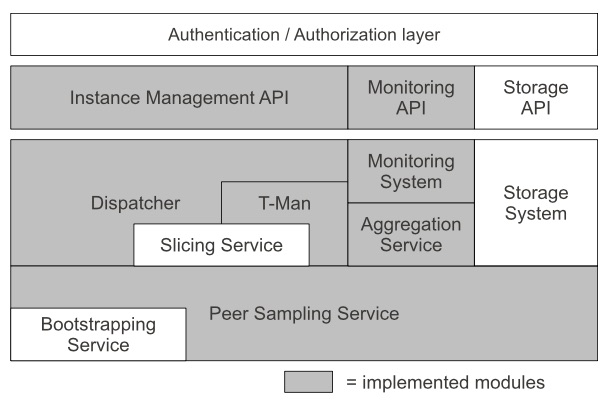
\includegraphics[width=125mm]{p2pcs_arch.jpg}
			\caption{P2P Cloud System Architecture\label{p2pcs_arch}}
		\end{figure}
	\end{center}
	
	We will briefly present each of the implemented modules (in gray).
	First the \textbf{Peer Sampling Service (PSS)} aims at providing each node with a list of peers to exchange 
	messages with. They achieve this by maintaining an unstructured overlay over the set of peers. It can 
	keep the overlay connected also in presence of churn, by using a simple gossip protocol. It uses a 
	BootStrapping Service to gather an initial set of nodes, although it not implemented yet; the current 
	implementation parses a text file with the IP addresses of the nodes.
	\\
	Second is the \textbf{Slicing Service (SS)}, which is used to rank the nodes according to one or more attributes, 
	it is also used to request slice of the whole cloud according to a user-defined criteria.
	\\
	Third is the \textbf{Aggregation Service (AS)}, which is used to compute global measures using local message 
	exchanges. It allows each peer to know system-wide parameters without the need to access a global registry.
	\\
	Fourth is the \textbf{Monitoring System}, which is implemented on top of the AS, and it collects global system 
	parameters and then provides them to the user. The MS API provides means to start and stop the display 
	of run-time instance informations. In the current implementation it is used to display the topology of 
	the network and the set of nodes of the slice a node belongs to.
	\\
	Fifth is the \textbf{T-Man component}, which is used to create a overlay network with a given topology, and it 
	is based on gossip protocols.
	\\
	Sixth is the \textbf{Dispatcher}, which is responsible for handling the requests submitted by the user through 
	the high level user interface and translate them into the appropriate low level gossip protocol 
	commands which are sent to the other nodes.
	\\
	Final is the \textbf{Instance Management API}, which contains all the functionalities to create and terminate 
	instances, and also to provide means to list which resources are held by this user.
	\\
	The implementation was done in Java, using the server-client paradigm.
	
	\subsubsection{Brief Analysis}
	It seems to be a dead project, since no updates were done or any changes were made since 2011. This 
	is one of the driving factors of this inquiry. Did support for this project stop out of disinterest 
	by the author, or did its tragic fate is the result of the coming to realization that it is not a 
	appropriate architecture for the Volunteer Cloud Infrastructure?
	
	The cornerstone of this architecture is the use of several gossip-based protocols to achieve such an 
	infrastructure. We need thus to analyze this design decision, in order to assess its effectiveness 
	with respect to particular problem that they are employed to solve.
	
	\subsubsection{Tentative....}
	P2PCS - Gossip-based protocols for large dynamic networks

	The Underlying incentive to use gossip-based protocol, in the context of V-Man 
	is to maximize the optimality of the VM's distribution in large scale networked 
	infrastructure, such as Clound infrastructure. The best visualization of this 
	specific problem is the following, from \cite{marzolla2011server}:
	
	\begin{center}
		\begin{figure}[h]
			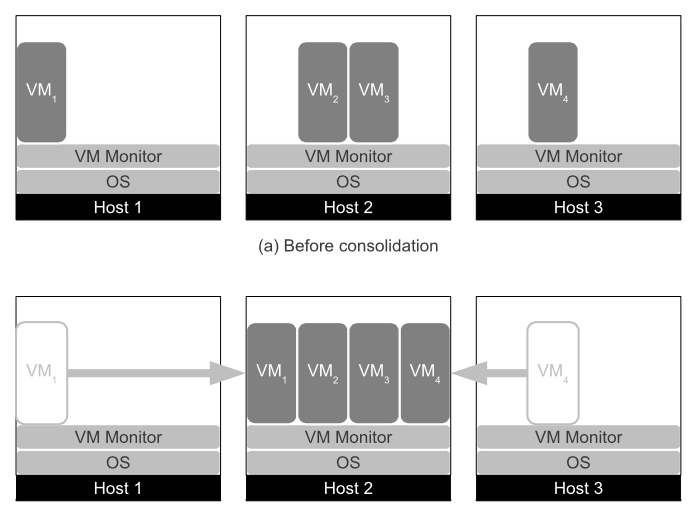
\includegraphics[width=125mm]{p2pcs_vm_aggregation.png}
			\caption{VM's aggregation problem\label{p2pcs_vm}}
		\end{figure}
	\end{center}
	
	We can formally 
	\section{Motivation}
	The motivation behind this proposal, is to analyze where past effort have not been as successful
	as expected. From this analysis, we wish to derive a design that take on past the shortcomings of 
	the previous attempts and venture to propose a viable implementation for this paradigm, which to 
	this day seems lacking.
	
	\subsection{Service Model}
	We need to situate where, within the already defined ontology of Cloud Computing, our effort will 
	focus. This effort focuses on the Platform-as-a-Service model, conversely to \cite{cathome}
	which attempted to propose a solution for all of the service models, and conversely to \cite{P2PCS} 
	that provides a solution w.r.t. the Infrastructure-as-a-Service model.
	\\
	The driving factor to focus on a PaaS model, is that we intend to propose a solution that does not 
	require any Hypervisor, and thus this solution will operate using Light Virtualization (in the form 
	of containers and more precisely groups \cite{cgroups}). Rather than providing an infrastructure on 
	which different VM can be deployed, we want to abstract this infrastructure by simply providing an 
	environment on which code can be executed, regardless of the underlying infrastructure.
	\\
	Although this implementation of the proof of concept targets the PaaS model, we will show at the end 
	that the underlying infrastructure that has been developed can be used in the context of SaaS also.
	
	\subsection{Applications}
	The C@H project presents 
	
	\section{Contributions}
	In this section we will present our novel contributions with respect to previous related work.
	
	\section{Overview of the Architecture}
	In this section we presents a high-level overview of the architecture that we developed to achieve 
	a fully de-centralized Volunteer Cloud Computing Infrastructure.
	\\
	\begin{center}
		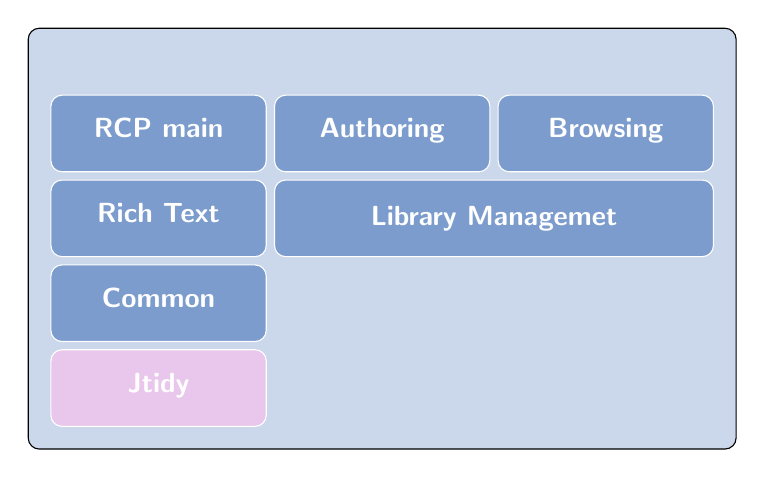
\begin{tikzpicture}[node distance=3pt,outer sep=0pt,
		blueb/.style={
		  draw=white,
		  fill=mybluei,
		  rounded corners,
		  text width=2.5cm,
		  font={\sffamily\bfseries\color{white}},
		  align=center,
		  text height=12pt,
		  text depth=9pt},
		greenb/.style={blueb,fill=mygreen},
		]
		\node[blueb] (RCP) {RCP main};
		\node[blueb,right=of RCP] (Aut) {Authoring};
		\node[blueb,right=of Aut] (Bro) {Browsing};
		\node[blueb,below=of RCP] (RTe) {Rich Text};
		\widernode{Aut}{Bro}{Library Managemet}{LMa}
		\node[blueb,below=of RTe] (Com) {Common};
		\node[blueb,fill=mypink,below=of Com] (Jti) {Jtidy};
		\begin{pgfonlayer}{background}
		\draw[blueb,draw=black,fill=mybluei!40] 
		  ([xshift=-\myframesep,yshift=3\myframesep]current bounding box.north west) 
		    rectangle 
		  ([xshift=\myframesep,yshift=-\myframesep]current bounding box.south east);
		\end{pgfonlayer}
		\end{tikzpicture}
	\end{center}
	
	\subsection{Network Layer}
	The network layer is responsible in aggregating the different geo-disparate resources 
	and managing them under \emph{churn}. Due to its highly dynamic nature, peer-to-peer 
	infrastructures are required to tolerate frequent churn, and this can compromise their 
	QoS unless the underlying networking structure is adequate (use of redundancy, replication, 
	and other means to operate under failures). Churn rate, is used to represent the frequency 
	of departure of participants with respect to the networking structure. Several options and 
	techniques are available to deal with the characteristics of peer-to-peer networks, lets 
	take a brief look at which one were adopted in the case of Cloud@Home and P2PCS; to help 
	us make an educated decision on which technique is more appropriate in our case.
	
	\subsubsection{Cloud@Home}
	They admit the need of a centralized entity to deal with the problems that arises from 
	utilizing distributed resources, thus they do not elaborate on how to overcome these 
	specific problems. Rather they justify the need for some centralized authority to guarantee 
	a decent level of QoS, in which they define \emph{decent} through their business model. 
	Finally, although they do use distributed heterogeneous resources, they compensate for 
	their high volatility by proposing premium means to securing resources. 
	
	\subsubsection{P2PCS}
	In the context of P2PCS, they point out the fact that they propose a \emph{fully de-centralized 
	peer-to-peer infrastructure} compared to their counterpart (C@H). They claim to achieve this via 
	several gossip-based protocols, and thus we must analyze their claims and justification to see 
	if we should use a comparable approach in our architecture.
	
	First let's introduce a very elementary definition of a gossip-based protocol
	
	
	\clearpage

\bibliographystyle{te}
\bibliography{bibliography}

\end{document}  